\documentclass[dvipsnames, hidelinks]{beamer}

% Enables the use of colour.
\usepackage{xcolor}
% Syntax high-lighting for code. Requires Python's pygments.
\usepackage{minted}
% Enables the use of umlauts and other accents.
\usepackage[utf8]{inputenc}
% Diagrams.
\usepackage{tikz}
% Settings for captions, such as sideways captions.
\usepackage{caption}
% Symbols for units, like degrees and ohms.
\usepackage{gensymb}
% Latin modern fonts - better looking than the defaults.
\usepackage{lmodern}
% Allows for columns spanning multiple rows in tables.
\usepackage{multirow}
% Better looking tables, including nicer borders.
\usepackage{booktabs}
% More math symbols.
\usepackage{amssymb}
% More math layouts, equation arrays, etc.
\usepackage{amsmath}
% More math fonts, like mathbb.
\usepackage{amsfonts}
% More theorem environments.
\usepackage{amsthm}
% More column formats for tables.
\usepackage{array}
% Adjust the sizes of box environments.
\usepackage{adjustbox}
% Better looking single quotes in verbatim and minted environments.
\usepackage{upquote}
% Better blank space decisions.
\usepackage{xspace}
% Better looking tikz trees.
\usepackage{forest}
% URLs.
\usepackage{hyperref}
% For plotting.
\usepackage{pgfplots}

% Various tikz libraries.
% For drawing mind maps.
\usetikzlibrary{mindmap}
% For adding shadows.
\usetikzlibrary{shadows}
% Extra arrows tips.
\usetikzlibrary{arrows.meta}
% Old arrows.
\usetikzlibrary{arrows}
% Automata.
\usetikzlibrary{automata}
% For more positioning options.
\usetikzlibrary{positioning}
% Creating chains of nodes on a line.
\usetikzlibrary{chains}
% Fitting node to contain set of coordinates.
\usetikzlibrary{fit}
% Extra shapes for drawing.
\usetikzlibrary{shapes}
% For markings on paths.
\usetikzlibrary{decorations.markings}
% For advanced calculations.
\usetikzlibrary{calc}

% GMIT colours.
\definecolor{gmitblue}{RGB}{20,134,225}
\definecolor{gmitred}{RGB}{220,20,60}
\definecolor{gmitgrey}{RGB}{67,67,67}

% Change some style options.
\usetheme{metropolis}
\usemintedstyle{manni}
\setbeamercolor{structure}{fg=gmitblue}
\setbeamercolor{frametitle}{fg=white, bg=gmitred}
\setbeamercolor{alerted text}{fg=gmitblue}
\usefonttheme[onlymath]{serif}

% \citeurl can be used to a clickable short url to a slide as a reference.
\renewcommand\footnoterule{}
\newcommand{\citeurl}[1]{\let\thefootnote\relax\footnotetext{\tiny \textcolor{gmitgrey}{\href{http://#1}{#1}}}}
\newcommand{\citeeg}[1]{\let\thefootnote\relax\footnotetext{\tiny \textcolor{gmitgrey}{#1}}}

% A basic horizontal rule.
\newcommand{\hr}{\rule{\textwidth}{0.5pt}}

% Prevent minted from showing errors.
\makeatletter
\expandafter\def\csname PYGdefault@tok@err\endcsname{\def\PYGdefault@bc##1{{\strut ##1}}}
\makeatother

\begin{document}
  \title{Non-deterministic Finite Automata}
  \subtitle{}
  \author{ian.mcloughlin@gmit.ie}
  \date{}

  \begin{frame}
    \titlepage
  \end{frame}

  
\begin{frame}{Non-determinism}
  \begin{description}
    \item[DFAs] always have exactly one state to transition to when in any given state and reading any given symbol.
    \vspace{4mm}
    \item[One arrow] emerging from each state for each symbol. (Sometimes we use one arrow for two symbols for tidiness.)
    \vspace{4mm}
    \item[Non-deterministic] finite automata can have any number of arrows for each state and symbol.
    \vspace{4mm}
    \item[Non-determinism] simplifies automata theory, and it can be shown that NFAs and DFAs recognise the same set of languages.
  \end{description}
\end{frame}


\begin{frame}[fragile]{NFA example}
  \begin{center}
    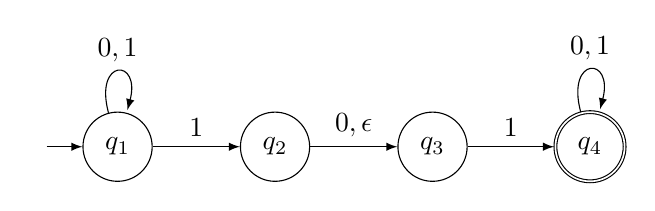
\begin{tikzpicture}[auto, on grid, node distance=2cm, initial text=, >=latex]
      \node[state, initial]   (q_1)                {$q_1$}; 
      \node[state]            (q_2) [right of=q_1] {$q_2$};
      \node[state]            (q_3) [right of=q_2] {$q_3$}; 
      \node[state, accepting] (q_4) [right of=q_3] {$q_4$};
      \path[->] 
        (q_1) edge [loop above] node {$0,1$}        ()
              edge []           node {$1$}          (q_2)
        (q_2) edge []           node {$0,\epsilon$} (q_3)
        (q_3) edge []           node {$1$}          (q_4)
        (q_4) edge [loop above] node {$0,1$}        ();
    \end{tikzpicture}
  \end{center}
  \begin{center}
    Try running the following strings on the automaton. \\
    $111101$, $00001010$, $1110$, $\epsilon$ \\
    Describe in words the strings that the automaton recognises.
  \end{center}
  \citeeg{Sipser page 48}
\end{frame}


\begin{frame}[fragile]{NFA example}
  \begin{center}
    Construct an NFA with alphabet $\{0, 1\}$ to recognise the language $\{ w| w \textrm{ ends with } 00\}$. Try to do it with only three states.
  \end{center}
  \begin{center}
    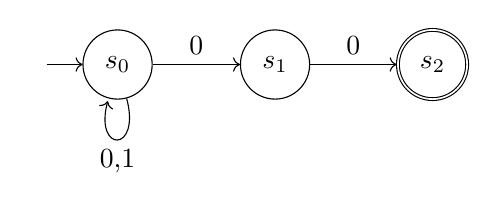
\begin{tikzpicture}[auto, on grid, node distance=2cm, initial text=]
      \node[state, initial]   (s_0)                {$s_0$};
      \node[state]            (s_1) [right of=s_0] {$s_1$};
      \node[state, accepting] (s_2) [right of=s_1] {$s_2$};
      \path[->]
        (s_0) edge [loop below] node {0,1} (s_0)
              edge []           node {0}   (s_1)
        (s_1) edge []           node {0}   (s_2);
    \end{tikzpicture}
  \end{center}
  \citeeg{Sipser Q 1.~7(a)}
\end{frame}


\begin{frame}[fragile]{Non-deterministic Finite Automaton (NFA) definition}
  An NFA is a 5-tuple $(Q,\Sigma,\delta,q_0,F)$ where
  \begin{description}
    \item[$Q$] is a finite set of \emph{states},
    \item[$\Sigma$] is a finite set called the \emph{alphabet},
    \item[$\delta$] is the \emph{transition function} ($Q \times \Sigma_{\epsilon} \rightarrow \mathcal{P}(Q)$),
    \item[$q_0$] is the \emph{start state} ($\in Q$), and
    \item[$F$] is the set of \emph{accept states} ($\subseteq Q$). 
  \end{description}
  \vspace{5mm}
  By $\Sigma_{\epsilon}$ we mean $\Sigma \cup \{ \epsilon \}$.
  e.g. When $\Sigma = \{0,1\}$, $\Sigma_{\epsilon} = \{\epsilon,0,1\}.$
  \citeeg{Sipser page 35}
\end{frame}

\begin{frame}[fragile]{Powerset example}

  Take any set, say $A = \{0,1,2\}$.
  Its powerset is the set of all its subsets, and is denoted $\mathcal{P}(A)$.


  $$
  \mathcal{P}(A) = \Big\{ \ 
                      \{ \} \  , \  \{ 0 \} \  , \  \{ 1 \} \  ,\   \{ 2 \} \  , \ 
                      \{ 0,1 \} \  , \  \{ 0,2 \} \  , \  \{ 1,2 \} \  , \ 
                      \{ 0,1,2 \} \ 
                    \Big\}
  $$


\end{frame} 
\end{document}
 